%-----------------------------------LICENSE------------------------------------%
%   This file is part of Mathematics-and-Physics.                              %
%                                                                              %
%   Mathematics-and-Physics is free software: you can redistribute it and/or   %
%   modify it it under the terms of the GNU General Public License as          %
%   published by the Free Software Foundation, either version 3 of the         %
%   License, or (at your option) any later version.                            %
%                                                                              %
%   Mathematics-and-Physics is distributed in the hope that it will be useful, %
%   but WITHOUT ANY WARRANTY; without even the implied warranty of             %
%   MERCHANTABILITY or FITNESS FOR A PARTICULAR PURPOSE.  See the              %
%   GNU General Public License for more details.                               %
%                                                                              %
%   You should have received a copy of the GNU General Public License along    %
%   with Mathematics-and-Physics.  If not, see <https://www.gnu.org/licenses/>.%
%------------------------------------------------------------------------------%

%   Use the standalone class for displaying the tikz image on a small PDF.
\documentclass[crop, tikz]{standalone}

%   Import the tikz package to use for the drawing.
\usepackage{tikz}

%   Load the arrows.meta library.
\usetikzlibrary{arrows.meta}

%   Begin the document.
\begin{document}

    %   Draw the figure.
    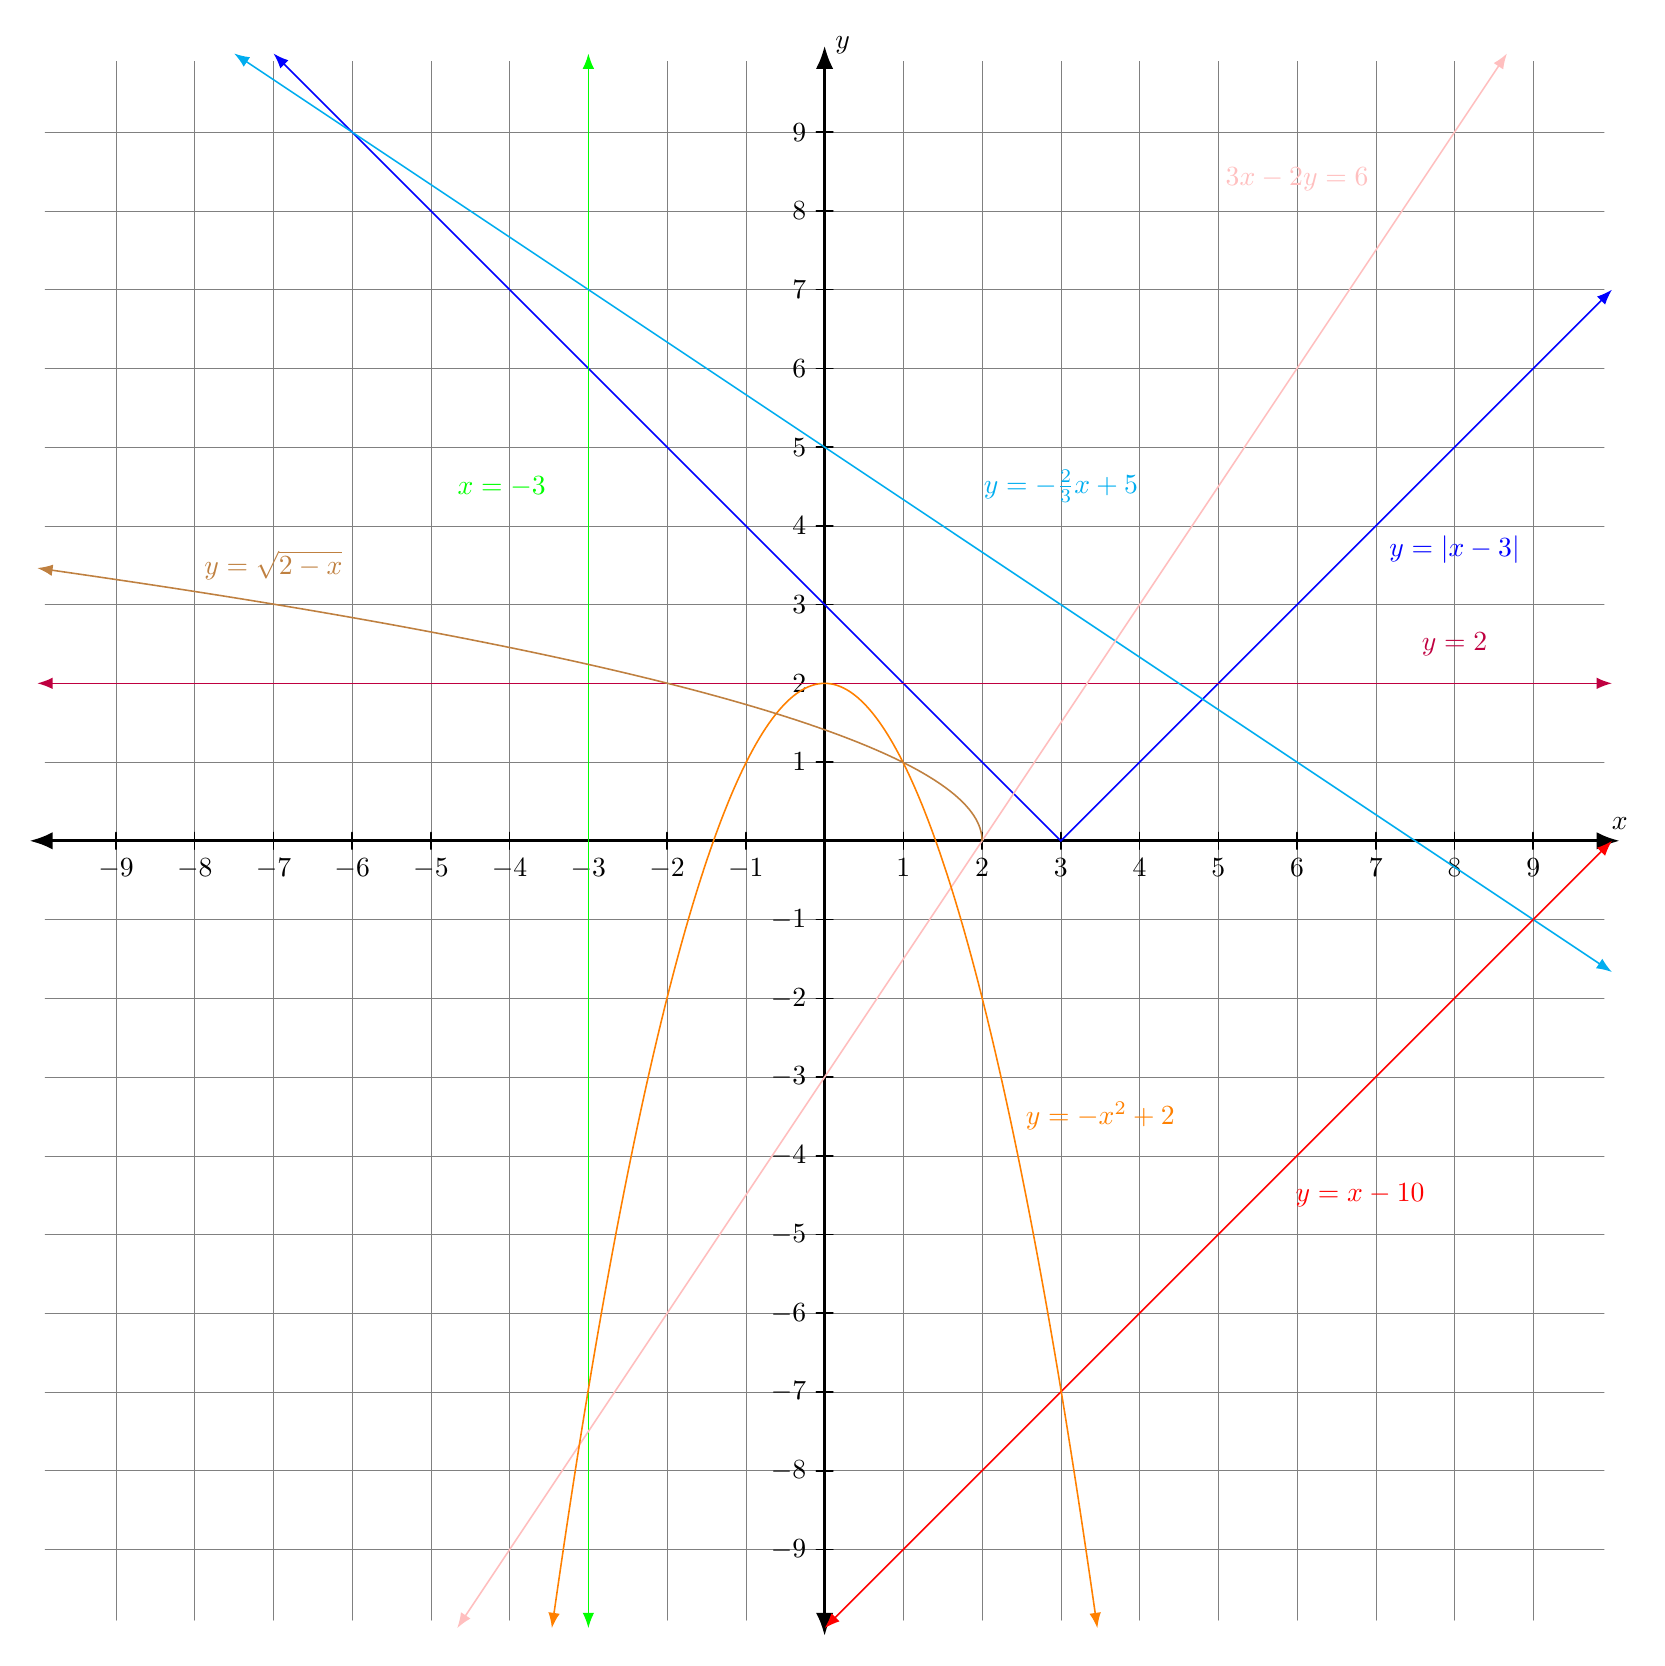
\begin{tikzpicture}[%
        >=Latex,
        line width=0.2mm,
        line cap=round
    ]
        % Draw a grid.
        \draw[style=help lines] (-9.9, -9.9) grid (9.9, 9.9);

        % Axes.
        \begin{scope}[very thick]
            \draw[<->] (-10.1, 0.0) to (10.1, 0.0) node [above] {$x$};
            \draw[<->] (0.0, -10.1) to (0.0, 10.1) node [right] {$y$};
        \end{scope}

        % Axes labels.
        \foreach\n in {1, 2, 3, 4, 5, 6, 7, 8, 9}{%
            \draw (\n, 3pt) to (\n, -3pt) node [below] {$\n$};
            \draw (-\n, 3pt) to (-\n, -3pt) node [below] {$-\n$};
            \draw (3pt, \n) to (-3pt, \n) node [left]  {$\n$};
            \draw (3pt, -\n) to (-3pt, -\n) node [left]  {$-\n$};
        }

        %   The absolute value function, |x - 3|.
        \draw[draw=blue, <->] (-7.0, 10.0) to (3.0, 0.0) to (10.0, 7.0);

        %   Several straight lines.
        \draw[draw=green, <->] (-3.0, -10.0) to (-3.0, 10.0);
        \draw[draw=purple, <->] (-10.0, 2.0) to (10.0, 2.0);
        \draw[draw=cyan, <->] (-7.5, 10.0) to (10.0, -1.667);
        \draw[draw=pink, <->] (-4.6666, -10.0) to (8.6666, 10.0);
        \draw[draw=red, <->] (0.0, -10.0) to (10.0, 0.0);

        %   A parabola.
        \draw[draw=orange, <->]
            (-3.4641, -10.0) parabola bend (0.0, 2.0) (3.4641, -10.0);

        %   And a square root function.
        \draw[rotate=90, shift={(0,-2)}, brown, ->]
            (0.0, 0.0) parabola bend (0.0, 0.0) (3.4641, 12.0);

        %   Label all of the functions.
        \node at (8.0, 3.7) {$\color{blue}y=|x-3|$};
        \node at (-4.1, 4.5) {$\color{green}x=-3$};
        \node at (8.0, 2.5) {$\color{purple}y=2$};
        \node at (3.0, 4.5) {$\color{cyan}{y=-\frac{2}{3}x+5}$};
        \node at (6.0, 8.4) {$\color{pink}3x-2y=6$};
        \node at (3.5, -3.5) {$\color{orange}y=-x^{2}+2$};
        \node at (6.8, -4.5) {$\color{red}y=x-10$};
        \node at (-7.0, 3.5) {$\color{brown}y=\sqrt{2-x}$};
    \end{tikzpicture}
\end{document}
